\documentclass{article}
\usepackage{pgfplots}
\pgfplotsset{compat=1.16}

\begin{document}

\begin{figure}[h]
    \centering
    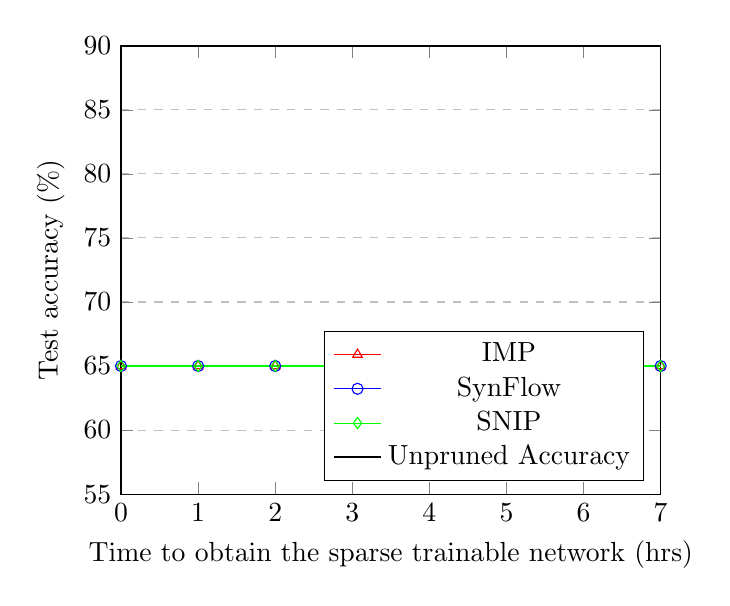
\begin{tikzpicture}
        \begin{axis}[
            xlabel={Time to obtain the sparse trainable network (hrs)},
            ylabel={Test accuracy (\%)},
            xmin=0, xmax=7,
            ymin=55, ymax=90,
            xtick={0,1,2,3,4,5,6,7},
            ytick={55,60,65,70,75,80,85,90},
            legend pos=south east,
            ymajorgrids=true,
            grid style=dashed,
        ]
        
        % IMP data
        \addplot[
            color=red,
            mark=triangle,
            ]
            coordinates {
                (0, 65)
                (1, 65)
                (2, 65)
                (3, 65)
                (4, 65)
                (5, 65)
                (6, 65)
                (7, 65)
            };
            \addlegendentry{IMP}
            
        % SynFlow data
        \addplot[
            color=blue,
            mark=o,
            ]
            coordinates {
                (0, 65)
                (1, 65)
                (2, 65)
                (3, 65)
                (4, 65)
                (5, 65)
                (6, 65)
                (7, 65)
            };
            \addlegendentry{SynFlow}
            
        % SNIP data
        \addplot[
            color=green,
            mark=diamond,
            ]
            coordinates {
                (0, 65)
                (1, 65)
                (2, 65)
                (3, 65)
                (4, 65)
                (5, 65)
                (6, 65)
                (7, 65)
            };
            \addlegendentry{SNIP}
            
        % Unpruned Accuracy
        \addplot[
            color=black,
            thick,
            ]
            coordinates {
                (0, 90)
                (1, 90)
                (2, 90)
                (3, 90)
                (4, 90)
                (5, 90)
                (6, 90)
                (7, 90)
            };
            \addlegendentry{Unpruned Accuracy}
            
        \end{axis}
    \end{tikzpicture}
    \caption{Comparing test accuracy of sparse networks derived using early pruning methods for AlexNet with 99.3\% parameters removed and trained on the CIFAR-10 dataset. The x-axis shows the time taken to obtain the sparse trainable network.}
    \label{fig:sparse_network_accuracy}
\end{figure}

\end{document}